%Beamer-Vorlage, v1.02

\documentclass{beamer}
\usepackage[T1]{fontenc}
\usepackage[utf8]{inputenc}
\usepackage[UKenglish]{babel}
\usepackage{graphicx}
\usepackage[osf]{libertine}
\usepackage{microtype}

\usetheme{Madrid} %dieser Wert stellt das generelle Thema der Präsentation ein: Einfach einen der folgenden Namen eintragen
%Themes ohne Navigationsleiste: Boadilla, Pittsburgh, Rochester, Madrid, AnnArbor
%Themes mit baumartiger Navigationsleiste: Antibes, JuanLesPins, Montepellier
%Themes mit Inhaltsverzeichnis auf jeder Seite: Berkley, PaloAlto, Goettingen, Marburg, Hannover
%Themes mit Mini-Frame-Navigation: Berlin, Ilmenau, Dresden, Darmstadt, Frankfurth, Singapore, Szeged
%Themes mit Abschnitt/Unterabschnitt-Gliederung: Copenhagen, Luebeck, Malmoe, Warsaw

%\useinnertheme{default}
%default, circles, rectangels, rounded, inmargin

%\useoutertheme{default}
%default, infolines, miniframe, smoothbars, sidebar, split, shadow, tree, smouthtree

\usecolortheme[RGB={36,110,188}]{structure} %mit dieser Zeile kann man eigene Farbstile vorgeben, oder man verwendet eine der Namen aus den drei folgenden Zeilen (die Farben sind aber eher gruselig als brauchbar!)
%vollstaendig: default, arbatross, beetle, crane, dove, fly, seagull, wolverine
%inner color theme: lilly, orchid, rose
%outer color theme: whale, seahorse, dolphin

\setbeamerfont{frametitle}{size=\normalsize} %Dieser Werk setzt die Schriftgröße des Framtitle fest (Standard ist etwas größer)

\title[Paläozoische Schildkröten Türkei]{Die paläozoischen Schildkröten der nordwestlichen Türkei}
\subtitle{Lebensweise und Fortpflanzung}
\date[Turtle 2012]{Tagung der Turtle-Fans 2012} %wenn man hier "\today" einträgt, bekommt man das aktuelle Datum
\author[Johnson et al.]{William Johnson\inst{1} \and Clark Hemmond\inst{1} \and Charly de Bronka\inst{2}}
\institute[Uni Haushagen]{
	\inst{1}Universität Haushagen, Abteilung für Schildkrötologie \and
	\inst{2}Turtle GmbH}
\titlegraphic{\includegraphics[height=1.5cm]{UniHaushagen.pdf} \hspace{1cm} \includegraphics[height=1.5cm]{Turtle.jpg}}

\begin{document}
\maketitle

\tableofcontents

%\part{Vorlesung 1} % mit "part" kann man seine Vorträge noch weiter gliedern, zum Beispiel für jede Vorlesung eine eigene mit jeweils eigenem Inhaltsverzeichnis und Struktur
\section{Einleitung}

\begin{frame}
	\frametitle{Verbreitung der Schildkröten}
	\begin{center}
	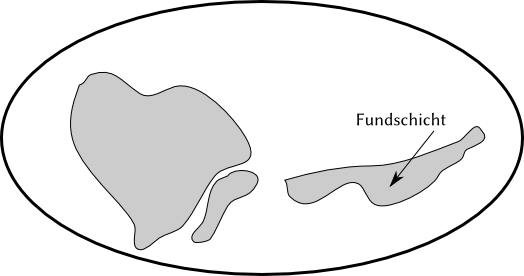
\includegraphics[width=0.7\textwidth]{Karte.png}
	
	{\small Die Weltkarte vor 400 Millionen Jahren. Links der Urkontinent, rechts seine Begleiter. Der Pfeil zeigt auf die Fundschicht der Schildkröten.}

	\end{center}
\end{frame}

\section{Spezieller Teil}
\subsection{Taxonomie}

\begin{frame}
	\frametitle{Schildkrötenarten}

	Es gibt insgesamt 20 bekannte Gattungen paläozoischer Schildkröten, sie treten stratigrafisch wie folgt auf:
	
	\begin{block}{Gattungen} %erzeugt einen einfachen Block
		\textit{Turtleiana brodeana}
		
		\textit{Comminsunia elegans}
		
		\textit{Joldia fingeri}
		
		\dots
	\end{block}

\end{frame}

\subsection{Ontogenie}

\begin{frame}
	\frametitle{Wie Schildkröten heranwachsen}

	Schildkröten sind Lebewesen, die durch viele Dinge beeinflusst werden, das sind zum Beispiel:
	
	\begin{exampleblock}{Dinge, die Schildis Heranwachsen beeinflussen} %Block für Beispiele
		Luftfeuchtigkeit
		
		Tageszeit
		
		Stellung des Saturn im Sternbild Schütze
	\end{exampleblock}

\end{frame}

\section{Zusammenfassung}

\begin{frame}
	\frametitle{Besonderheiten bei paläozoischen Schildkröten}
	
	\begin{itemize}
		\item sind viel schwerfälliger
		\item haben grüne Augen
		\item jedes Weibchen wirft stets 3 Jungen
	\end{itemize}
	
	\begin{alertblock}{Achtung!} %Block für Warnungen
		Es gibt Ausnahmen!
	\end{alertblock}
\end{frame}

\begin{frame}
	\frametitle{Wie war das mit der Geografie?}
	
	\begin{columns} %benutze die Column-Umgebung, um Text und Bild oder Text und Text nebeneinander darzustellen
		\column[c]{6cm} %erzeugt zentriert ausgerichtete Spalte mit 6 cm Breite
			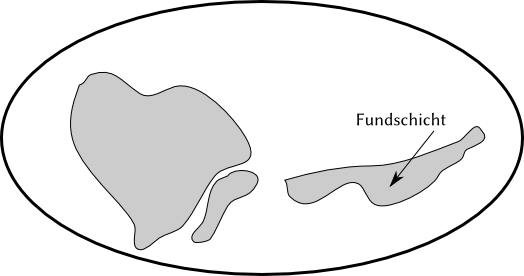
\includegraphics[height=3cm]{Karte.png}
		\column{.45\textwidth} %erzeugt eine Spalte, die 45 % der Textbreite einnimmt
			Kommen wir nochmal auf die Geografie zurück.
	\end{columns}	
\end{frame}

\section{Ende}

\begin{frame}
	\frametitle{Ende}
	\begin{center}
	Danke für die Aufmerksamkeit! -- Fragen? \vspace{0.3cm}

	
	{\footnotesize www.schildis.de}
	\end{center}
\end{frame}

\end{document}